% You should title the file with a .tex extension (hw1.tex, for example)
\documentclass[11pt]{article}

\usepackage{amsmath}
\usepackage{mathtools}
\usepackage{amssymb}
\usepackage{wrapfig}
\usepackage{fancyhdr}
\usepackage{tikz-qtree}
\usepackage{tikz-qtree-compat}
\usepackage[normalem]{ulem}
\usepackage{tikz}
\usepackage{graphicx}
\DeclareMathOperator*{\argmin}{argmin}
\DeclareMathOperator*{\argmax}{argmax}

\oddsidemargin0cm
\topmargin-2cm     %I recommend adding these three lines to increase the 
\textwidth16.5cm   %amount of usable space on the page (and save trees)
\textheight23.5cm  

\newcommand{\question}[2] {\vspace{.25in} \hrule\vspace{0.5em}
\noindent{\bf #1: #2} \vspace{0.5em}
\hrule \vspace{.10in}}
\renewcommand{\part}[1] {\vspace{.10in} {\bf (#1)}}
\linespread{1.5}

\newcommand{\myname}{Anonymous Authors}
\newcommand{\myhwnum}{12}

\setlength{\parindent}{0pt}
\setlength{\parskip}{5pt plus 1pt}
 
\DeclarePairedDelimiter\abs{\lvert}{\rvert}%

\pagestyle{fancyplain}

\begin{document}

\medskip                        % Skip a "medium" amount of space
                                % (latex determines what medium is)
                                % Also try: \bigskip, \littleskip

\thispagestyle{plain}
{\Large Statistical inference in theoretical models of cognition} \\
Sean, Agostina, Alex, Chunyu, Francesca, Srdjan, Carlos, Ken, and John

\section{Figures}
\clearpage

\begin{figure}
\begin{center}
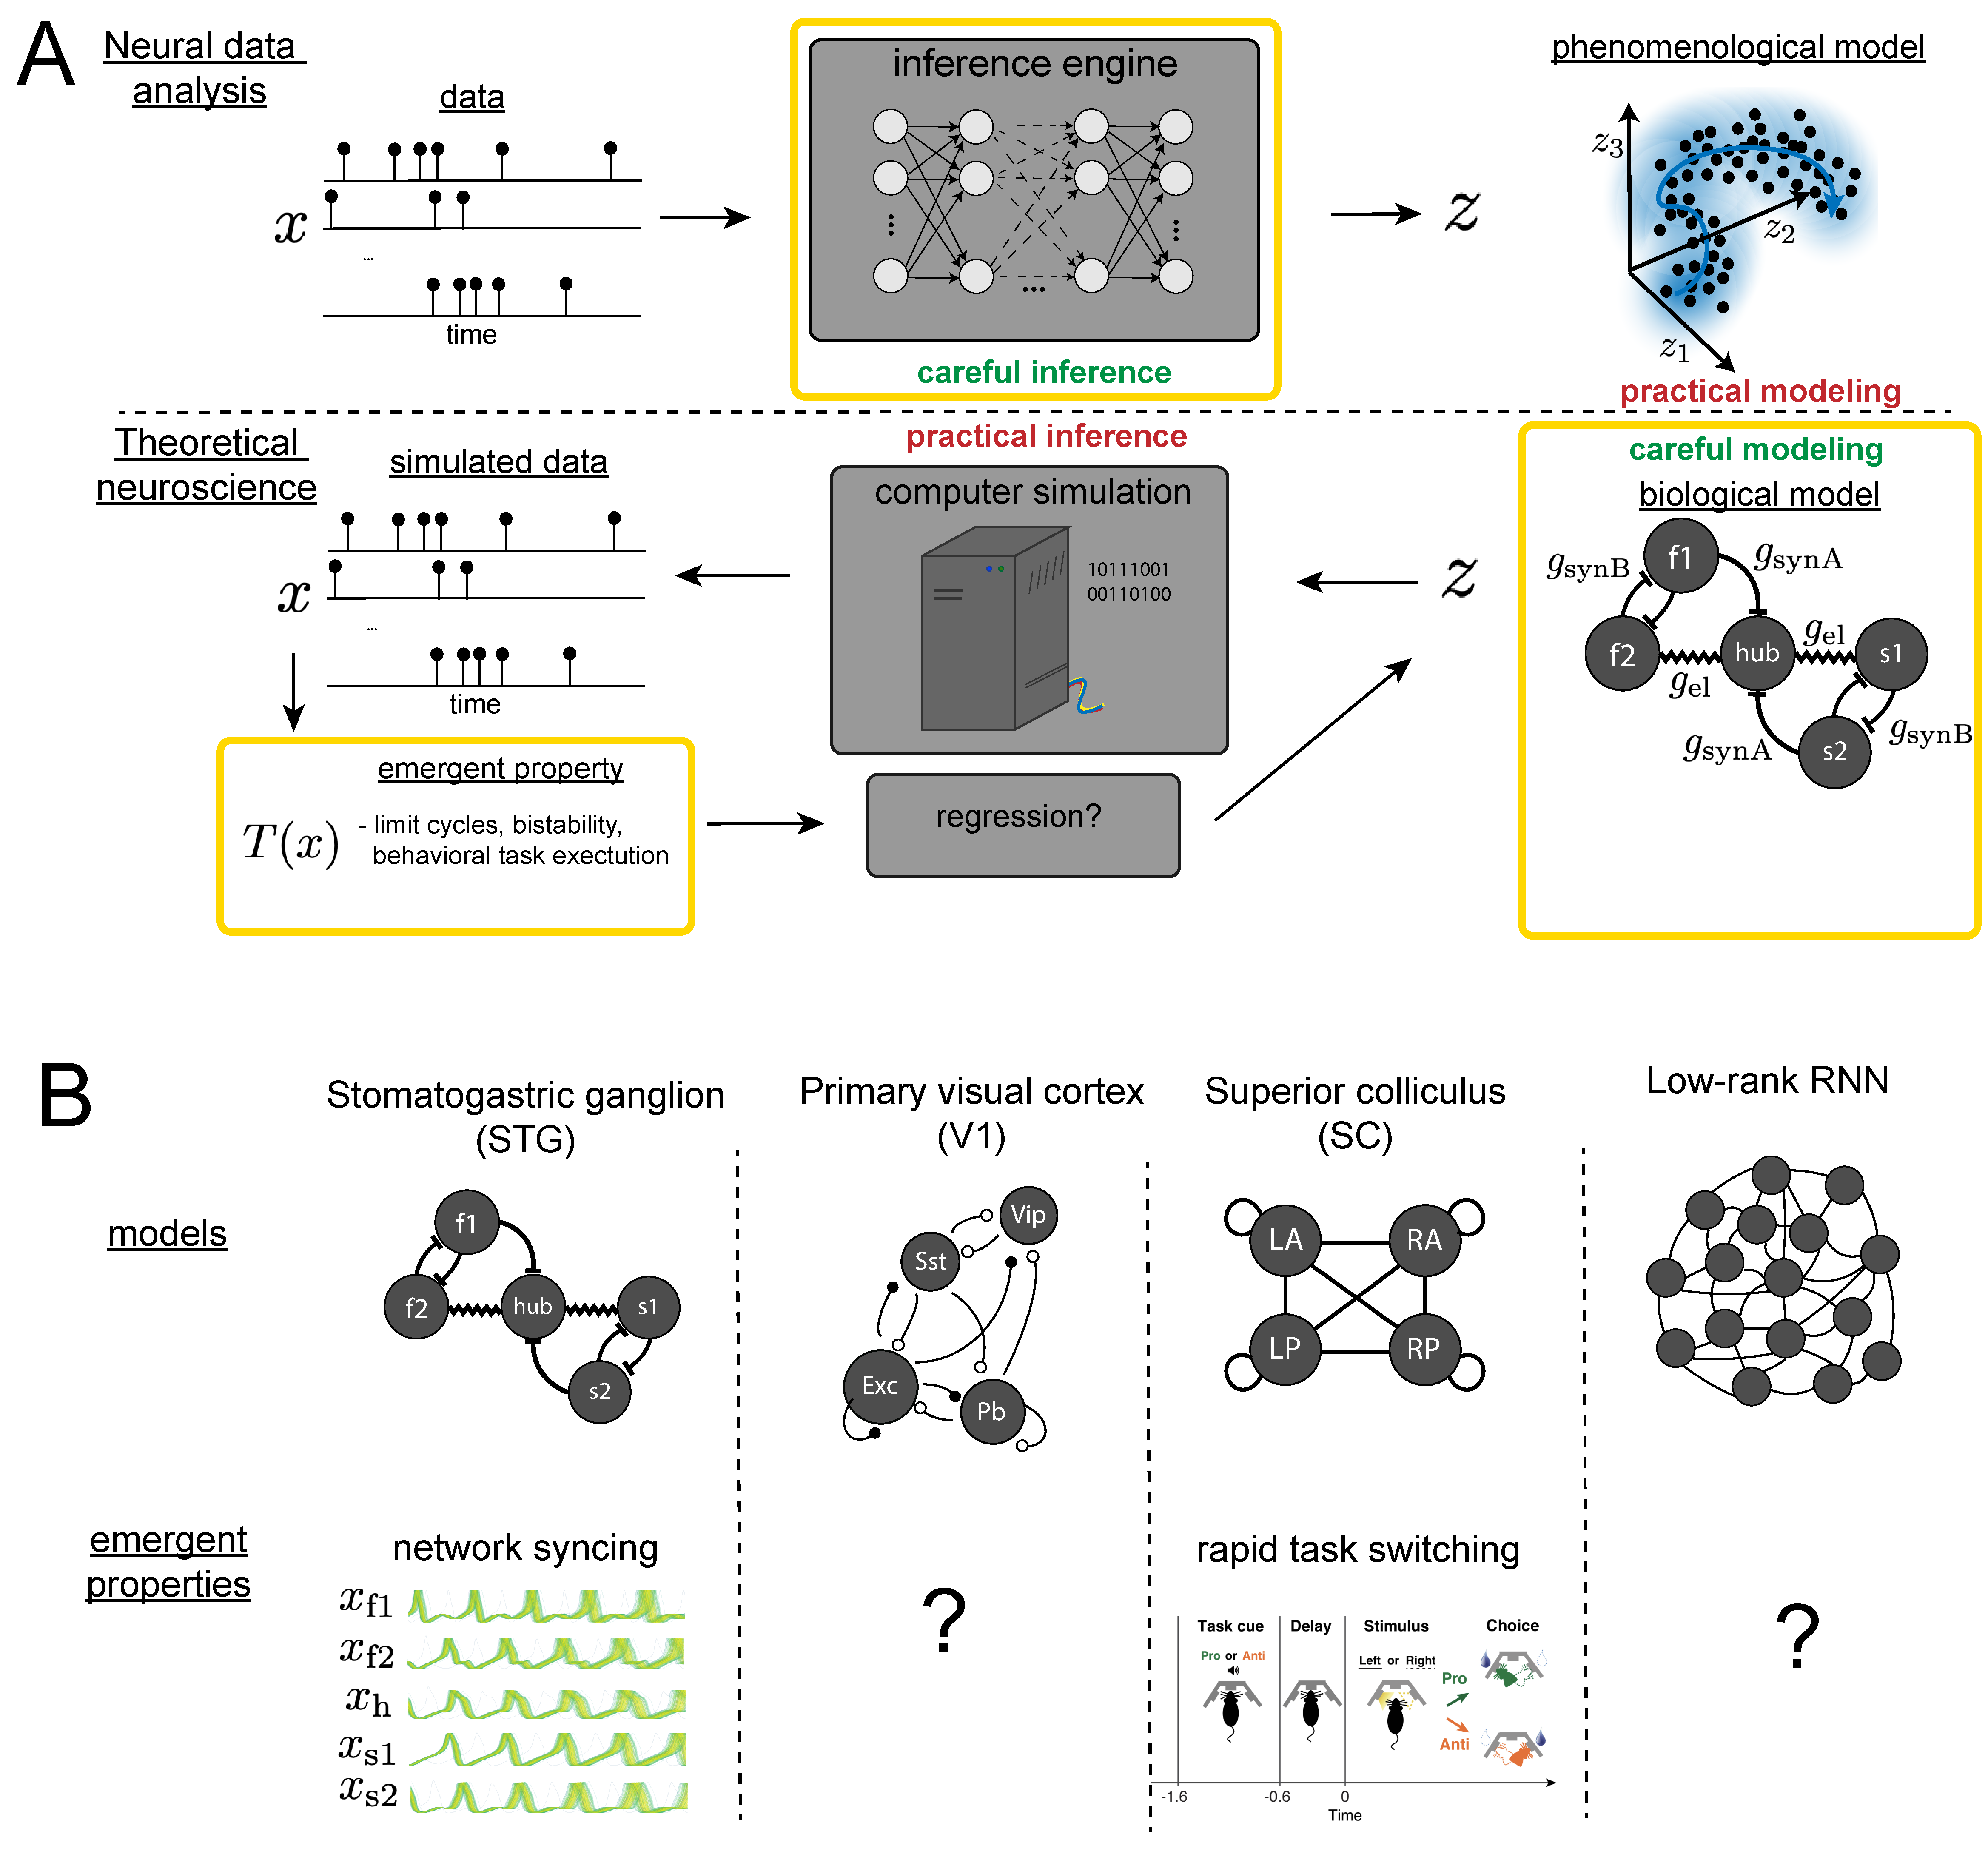
\includegraphics[scale=0.2]{figs/fig1/fig1.pdf}
\end{center}
\caption{\small A. \textit{Neural data analysis}: To identify structure in experimentally recorded neural data sets (left), neural data analysts use the modern inference engine (center) -- a collection of tools like convex optimization theory and deep learning from the machine learning literature -- to carefully execute Bayesian inference on a phenomenological generative model of the data.  Neural data analysts impose practical constraints to these phenomenological models so that Bayesian inference can be done. \textit{Theoretical Neuroscience}: Theoretical neuroscientists design systems of equations reflecting biological reality comprising a model (right, e.g. the STG) with the hopes of reproducing emergent properties of neural computation found in data (left).  In standard practice, models are evaluated by simulating them for many choices of parameters on a server (center).  To gain an understanding for how parameters of the model govern such emergent properties, theoretical neuroscientists are left to measure correlations or find other structure in the simulated activity. In this study, we introduce DSNs, which use the modern inference engine to learn distributions of model solutions given emergent properties of neural computations (yellow boxes).  B. We use DSNs to provide novel insights to popular models in theoretical neuroscience.  We examine network syncing in the STG, blah in a dynamic four neuron-type population model of primary visual cortex (V1), information routing in the superior colliculus (SC), and blah in low-rank recurrent neural networks (RNNs).}
\end{figure}

\clearpage

\begin{figure}
\begin{center}
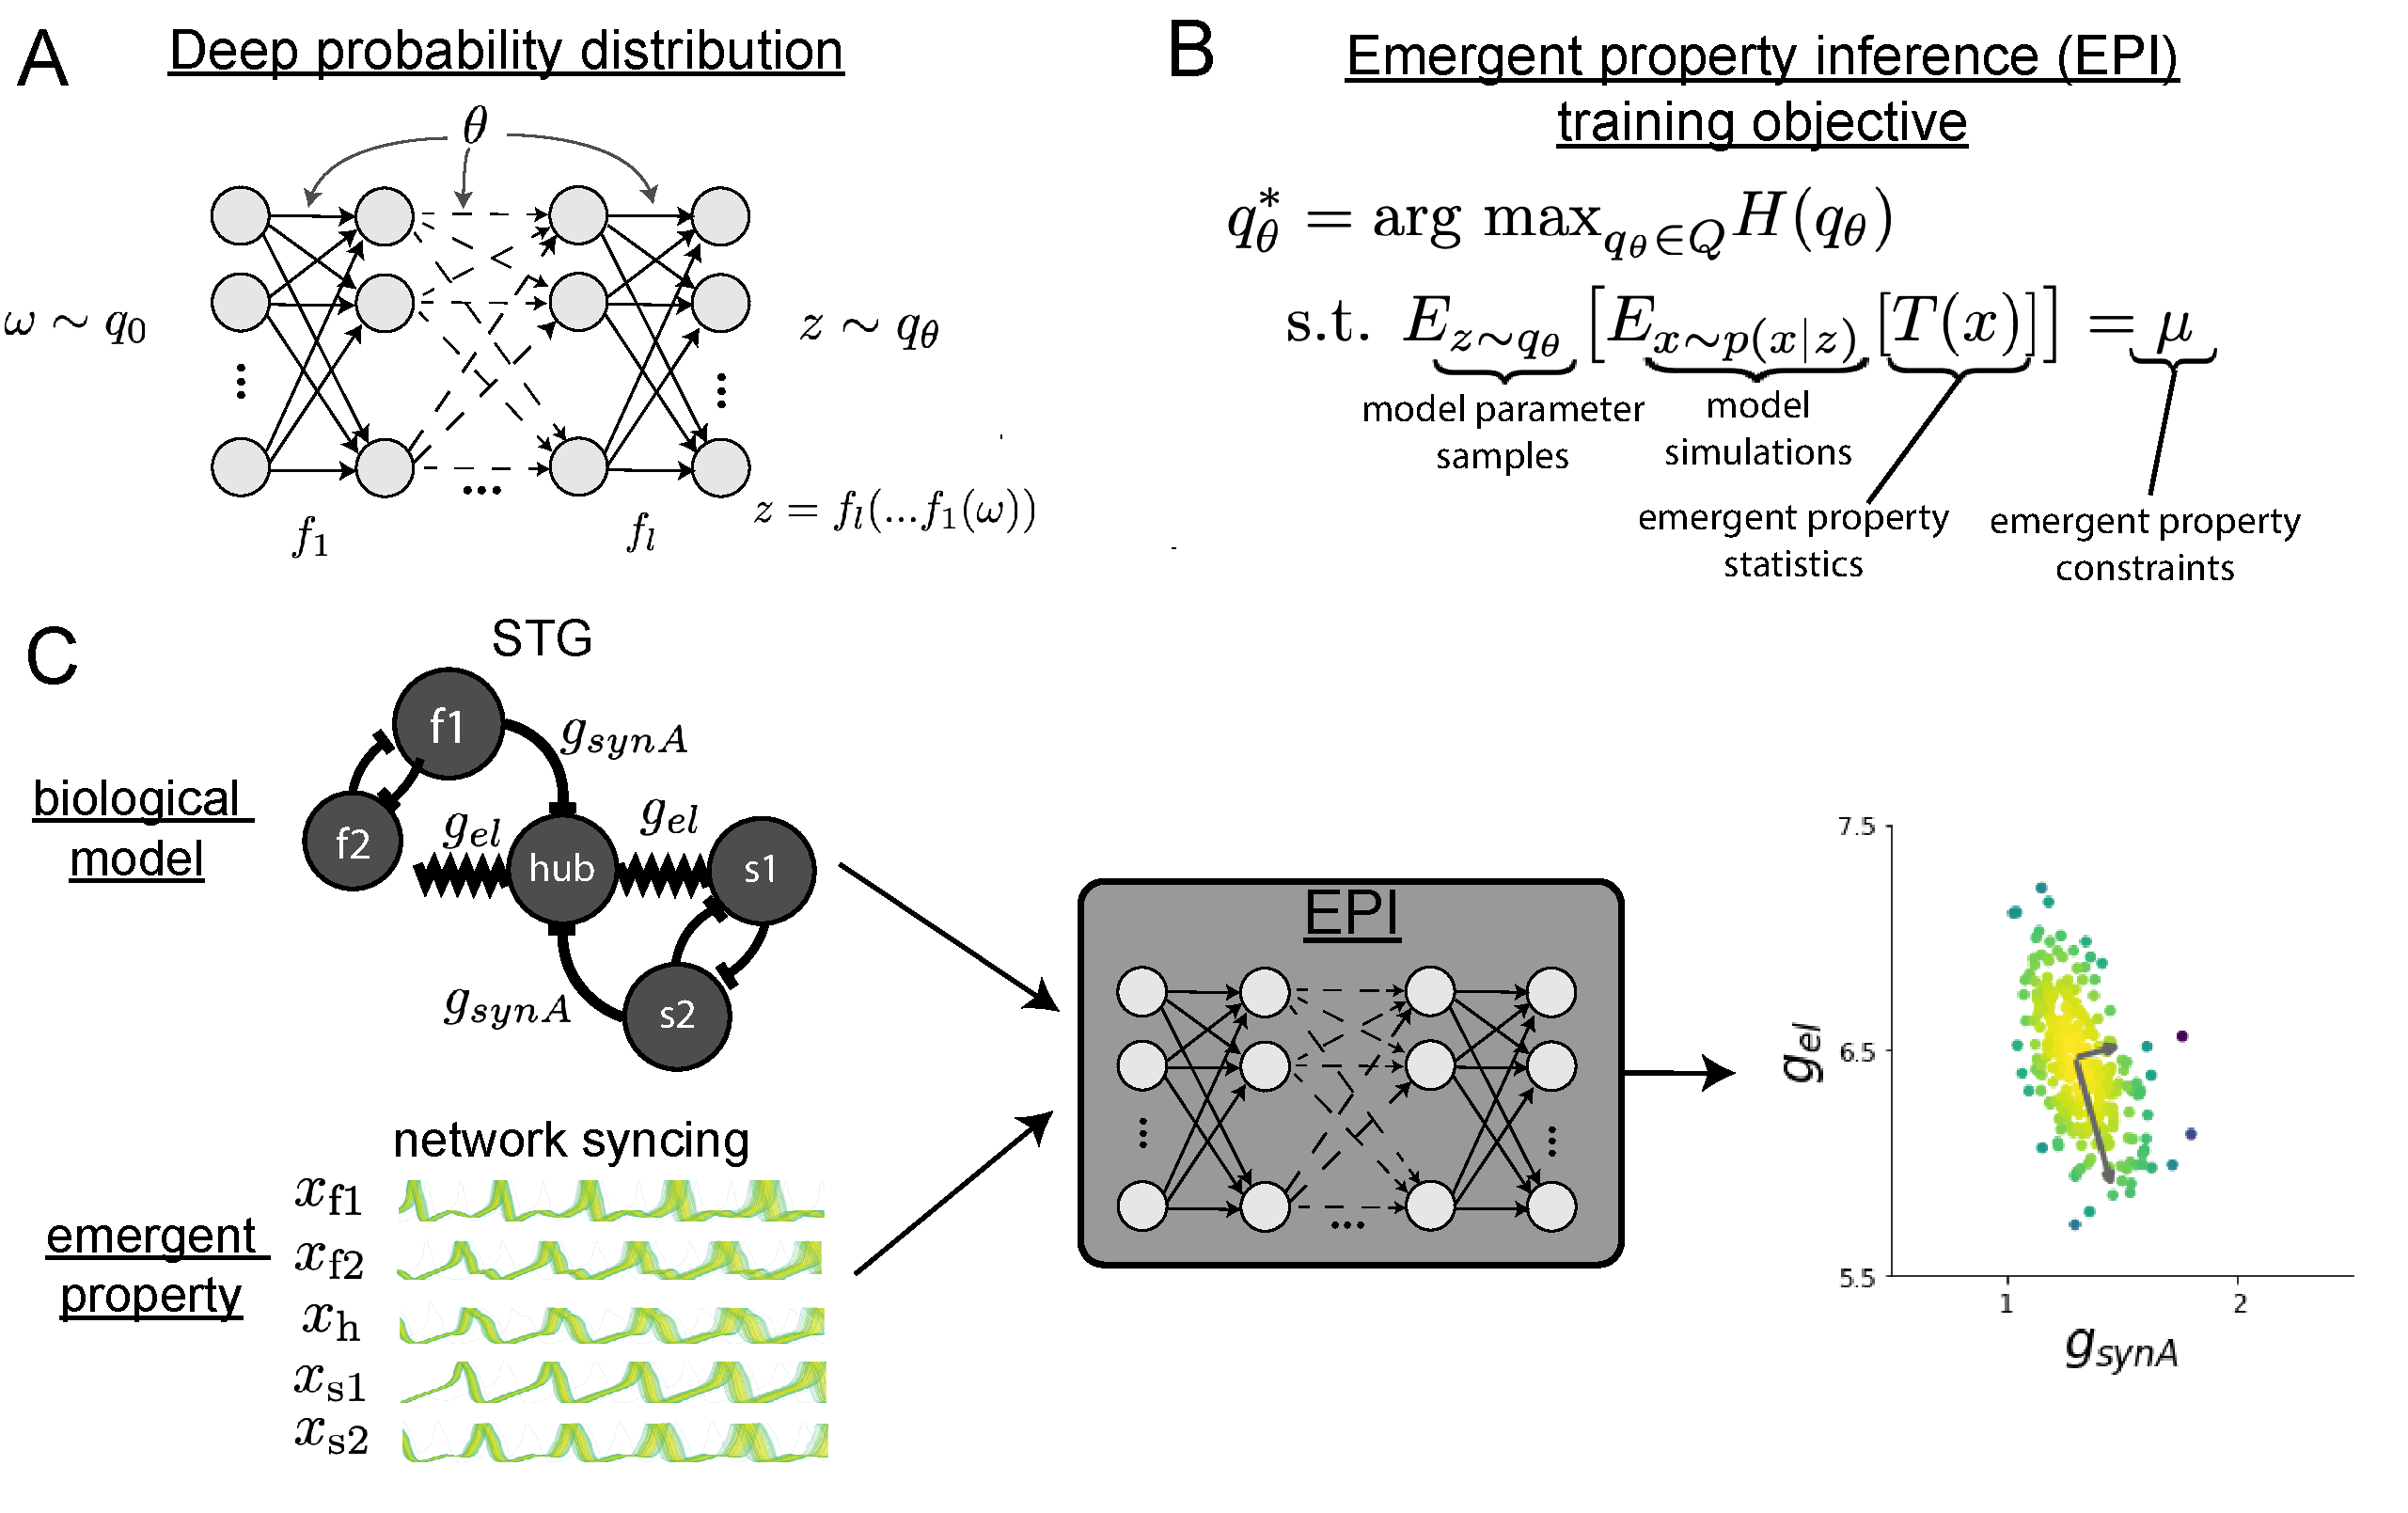
\includegraphics[scale=0.4]{figs/fig2/fig2.pdf}
\end{center}
\caption{A. Degenerate solution networks (DSNs) are deep probability distributions $q_\theta(z)$ of theoretical model parameterizations that produce emergent properties of interest.  The stochasticity of a deep probability distribution comes from a simple random variable $\omega \sim q_0$, where $q_0$ is often chosen to be an isotropic gaussian, and the structure comes from the deterministic transformation made by the deep neural network with optimized parameters $\theta$.  DSNs are the result of a constrained stochastic optimization, in which emergent properties $T(x)$ are fixed in expectation over model simulations $x \sim p(x \mid z)$ and DSN samples $z \sim q_\theta(z)$ to be a particular value $\mu$.  DSNs distributions maximize randomness through entropy. B. For a choice of model (STG) and emergent property (network syncing), a DSN learns a posterior distribution of the model parameters  $z = \left[g_{\text{el}}, g_{\text{synA}} \right]^\top$ conditioned on network syncing.}
\textbf{SB Comment}: In A, we have gaussian noise being fed into the deep probability distribution, and in B, we have a choice of model and emergent property predicating what the DSN is going to do.  There should be a way to depict these ideas without creating confusion on what the input to the DSN is.
\end{figure}

\clearpage

\begin{figure}
\begin{center}
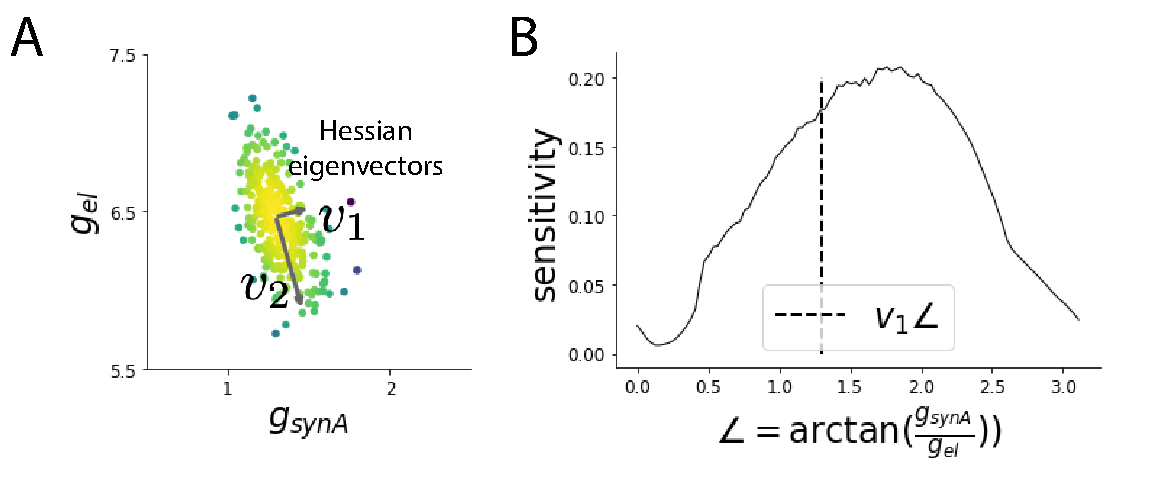
\includegraphics[scale=0.7]{figs/figS1/figS1.pdf}
\end{center}
Fig. S1: A. DSN distribution of STG model parameters producing network syncing.  B. Sensitivity of the system with respect to network syncing along all dimensions of parameter space away from the mode.
\end{figure}

\clearpage

\begin{figure}
\begin{center}
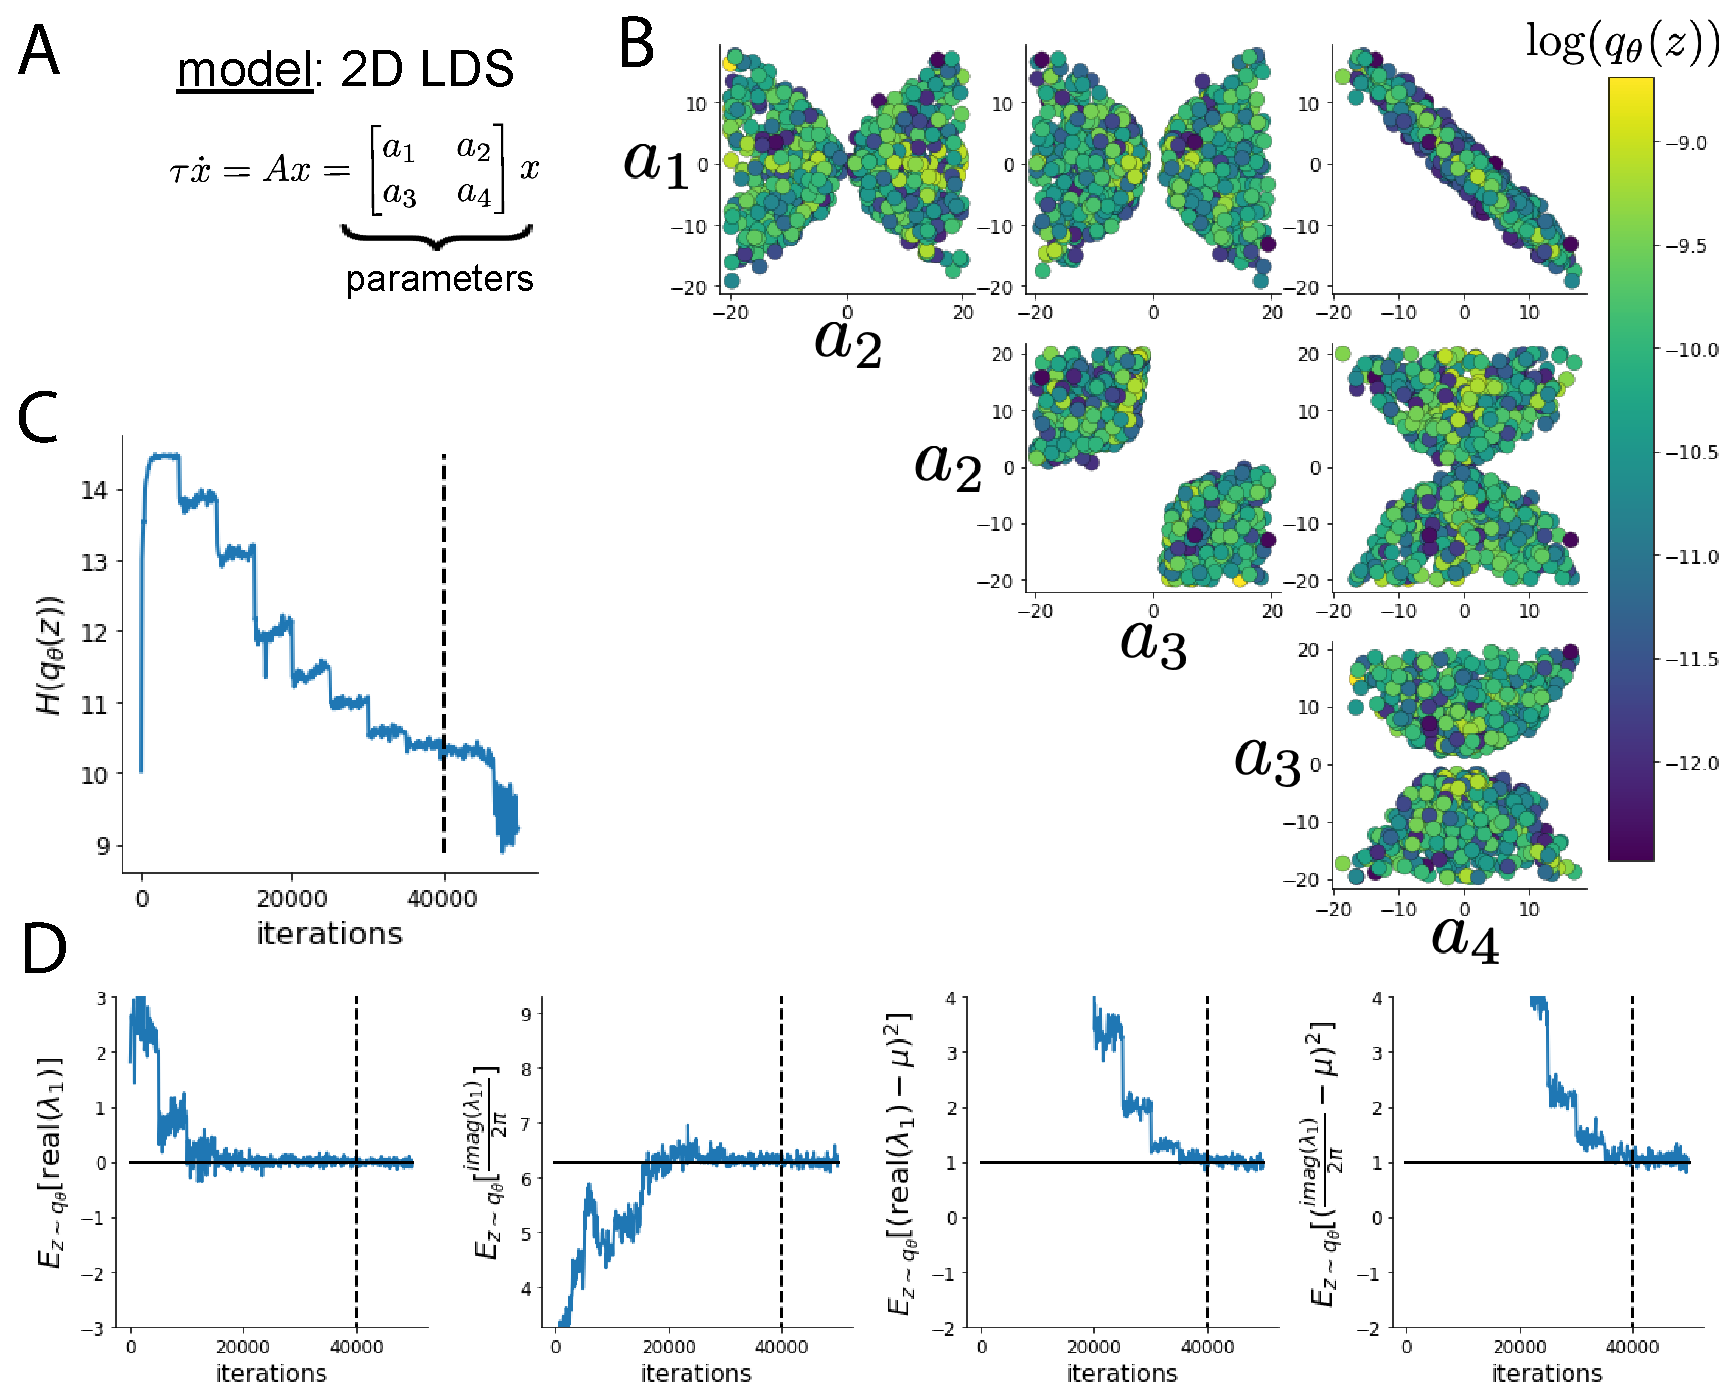
\includegraphics[scale=0.5]{figs/figS2/figS2.pdf}
\end{center}
Fig. S2: A. Two-dimensional linear dynamical system model, where real entries of the dynamics matrix $A$ are the parameters.  B. The DSN distribution for a 2D LDS with $\tau=1$ that produces an average of 1Hz oscillations with some small amount of variance.  C. Entropy throughout the optimization.  At the beginning of each augmented lagrangian epoch (5,000 iterations), the entropy dips due to the shifted optimization manifold where emergent property constraint satisfaction is increasingly weighted.  D. Emergent property moments throughout optimization.  At the beginning of each augmented lagrangian epoch, the emergent property moments move closer to their constraints.
\end{figure}

\clearpage

\begin{figure}
\begin{center}
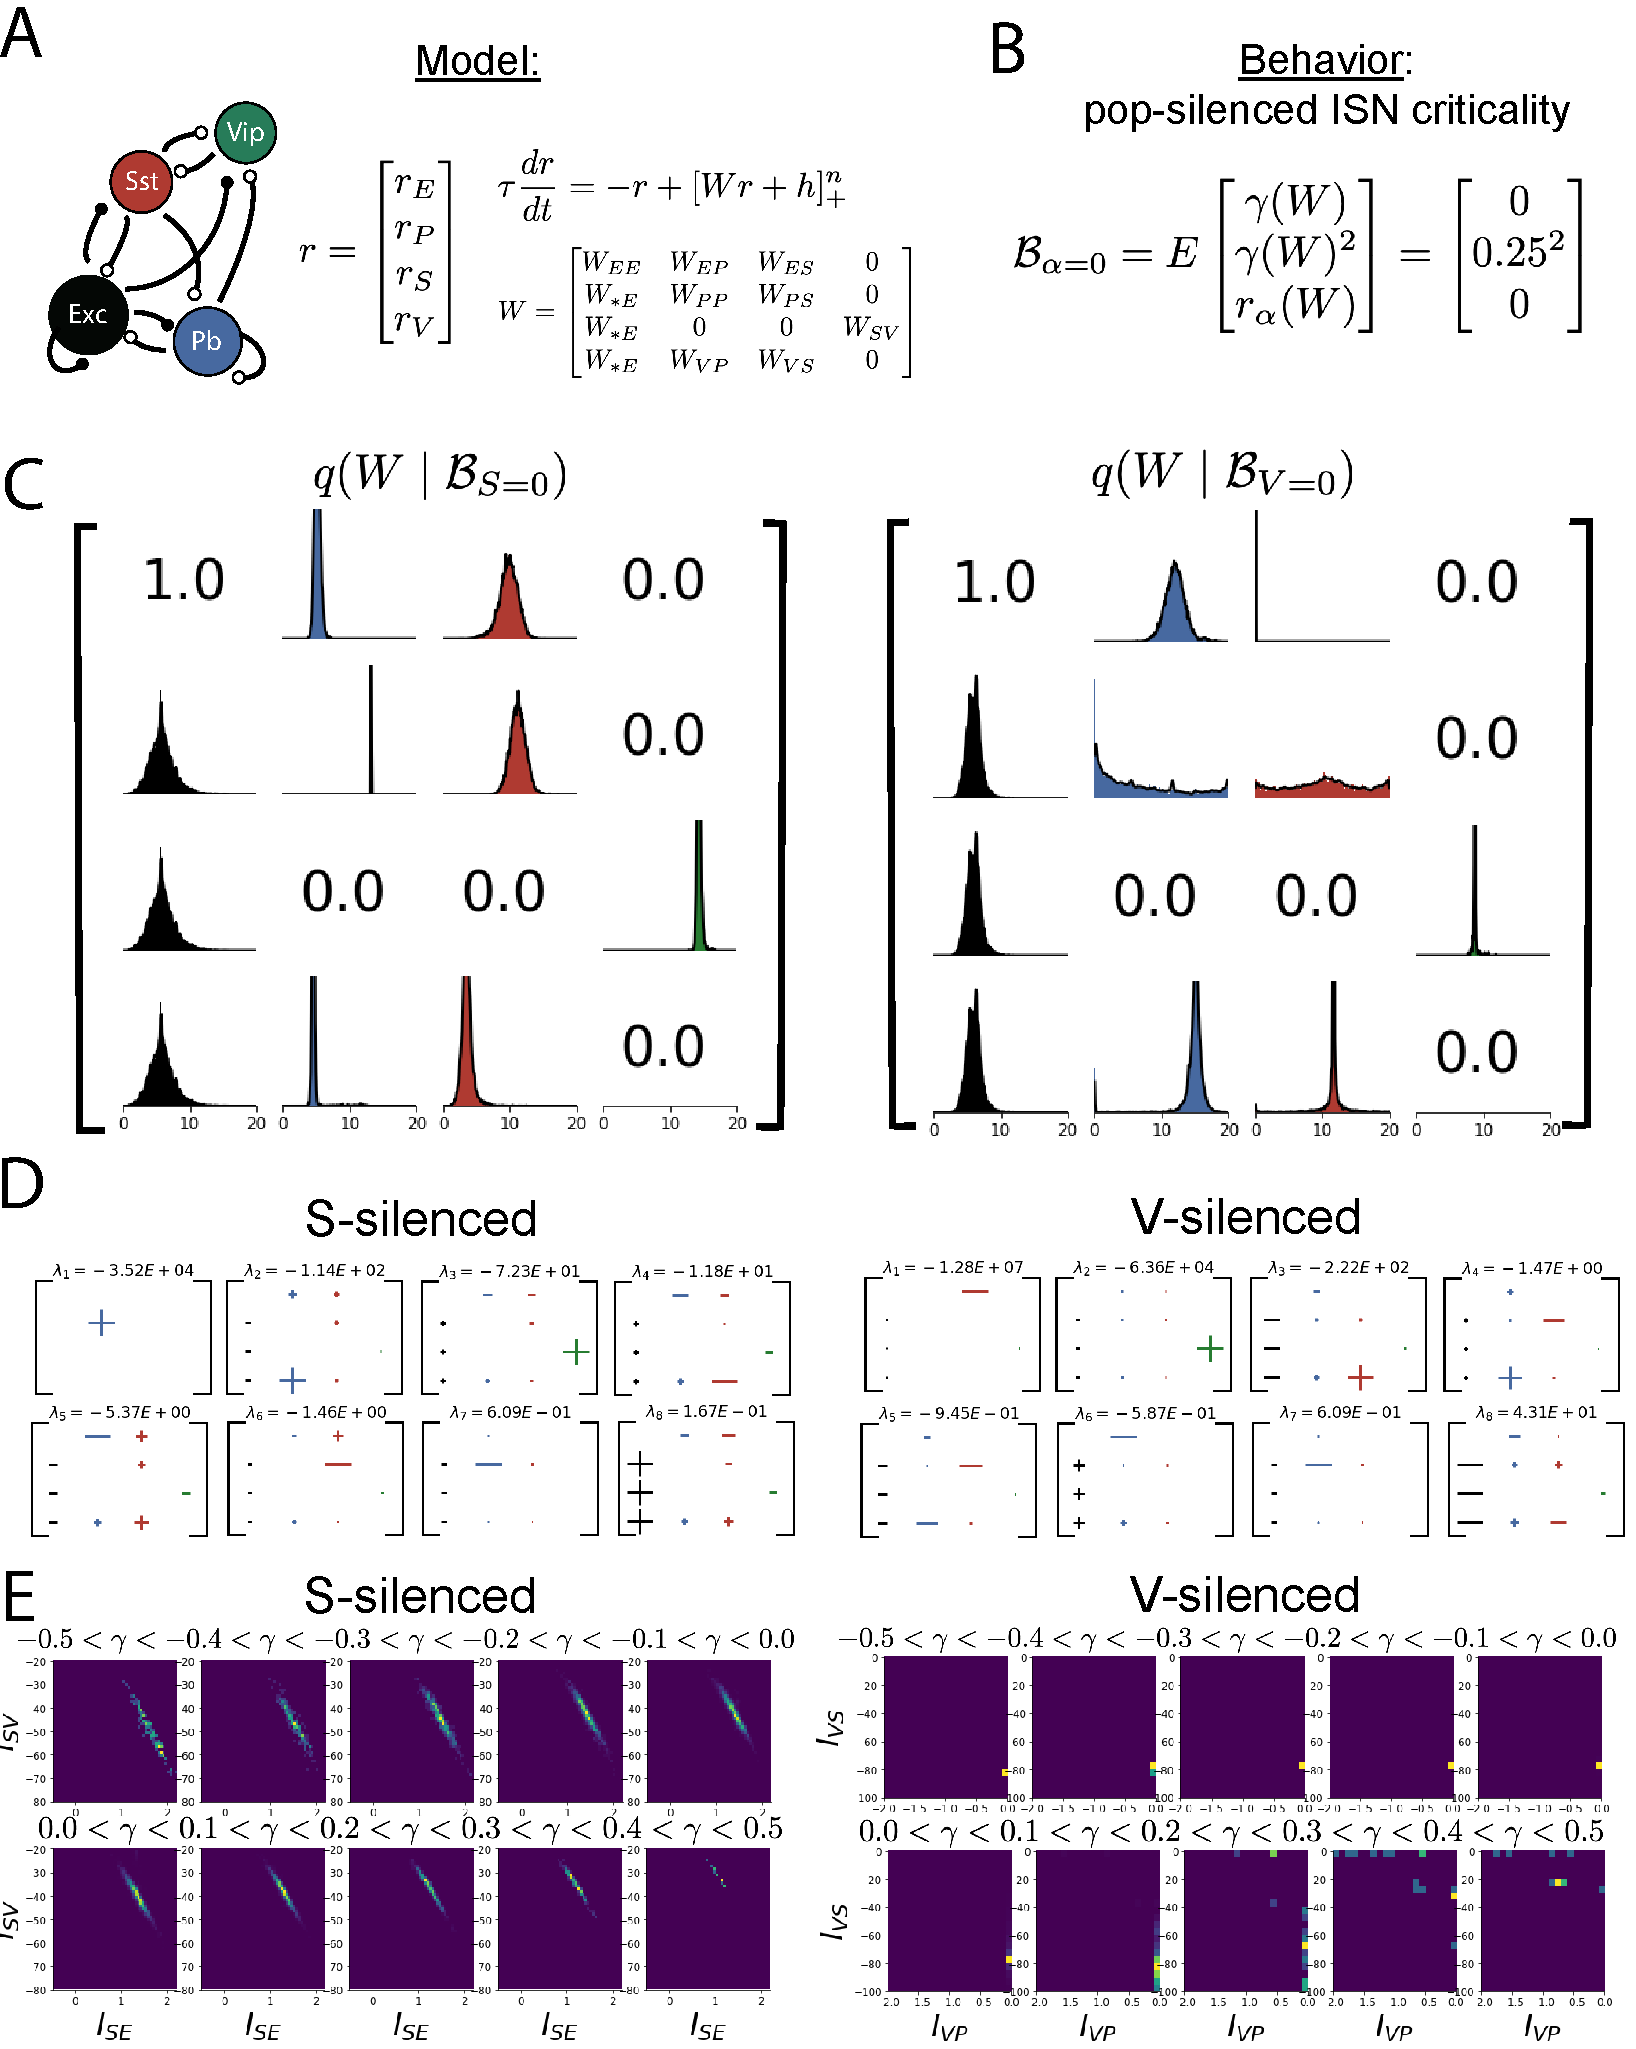
\includegraphics[scale=0.5]{models/V1/V1_Fig/V1_Fig.pdf}
\end{center}
\caption{\protectA.) Model of primary visual cortex (V1) Neurons: E (black), P (blue), S (red), and V (green).  Parameters: weights of the dynamics matrix $W$.  B.) The DSNs are conditioned on population-silenced ISN criticality.  C.) DSN distribution of the parameters of the V1 model conditioned on population-silened ISN criticality.  D.) Eigenmodes of the hessian of each DSN ordered by eigenvalue.  E. Input to silenced population across ISN regimes of the DSN posterior.
}
\end{figure}

\clearpage

\begin{figure}
\begin{center}
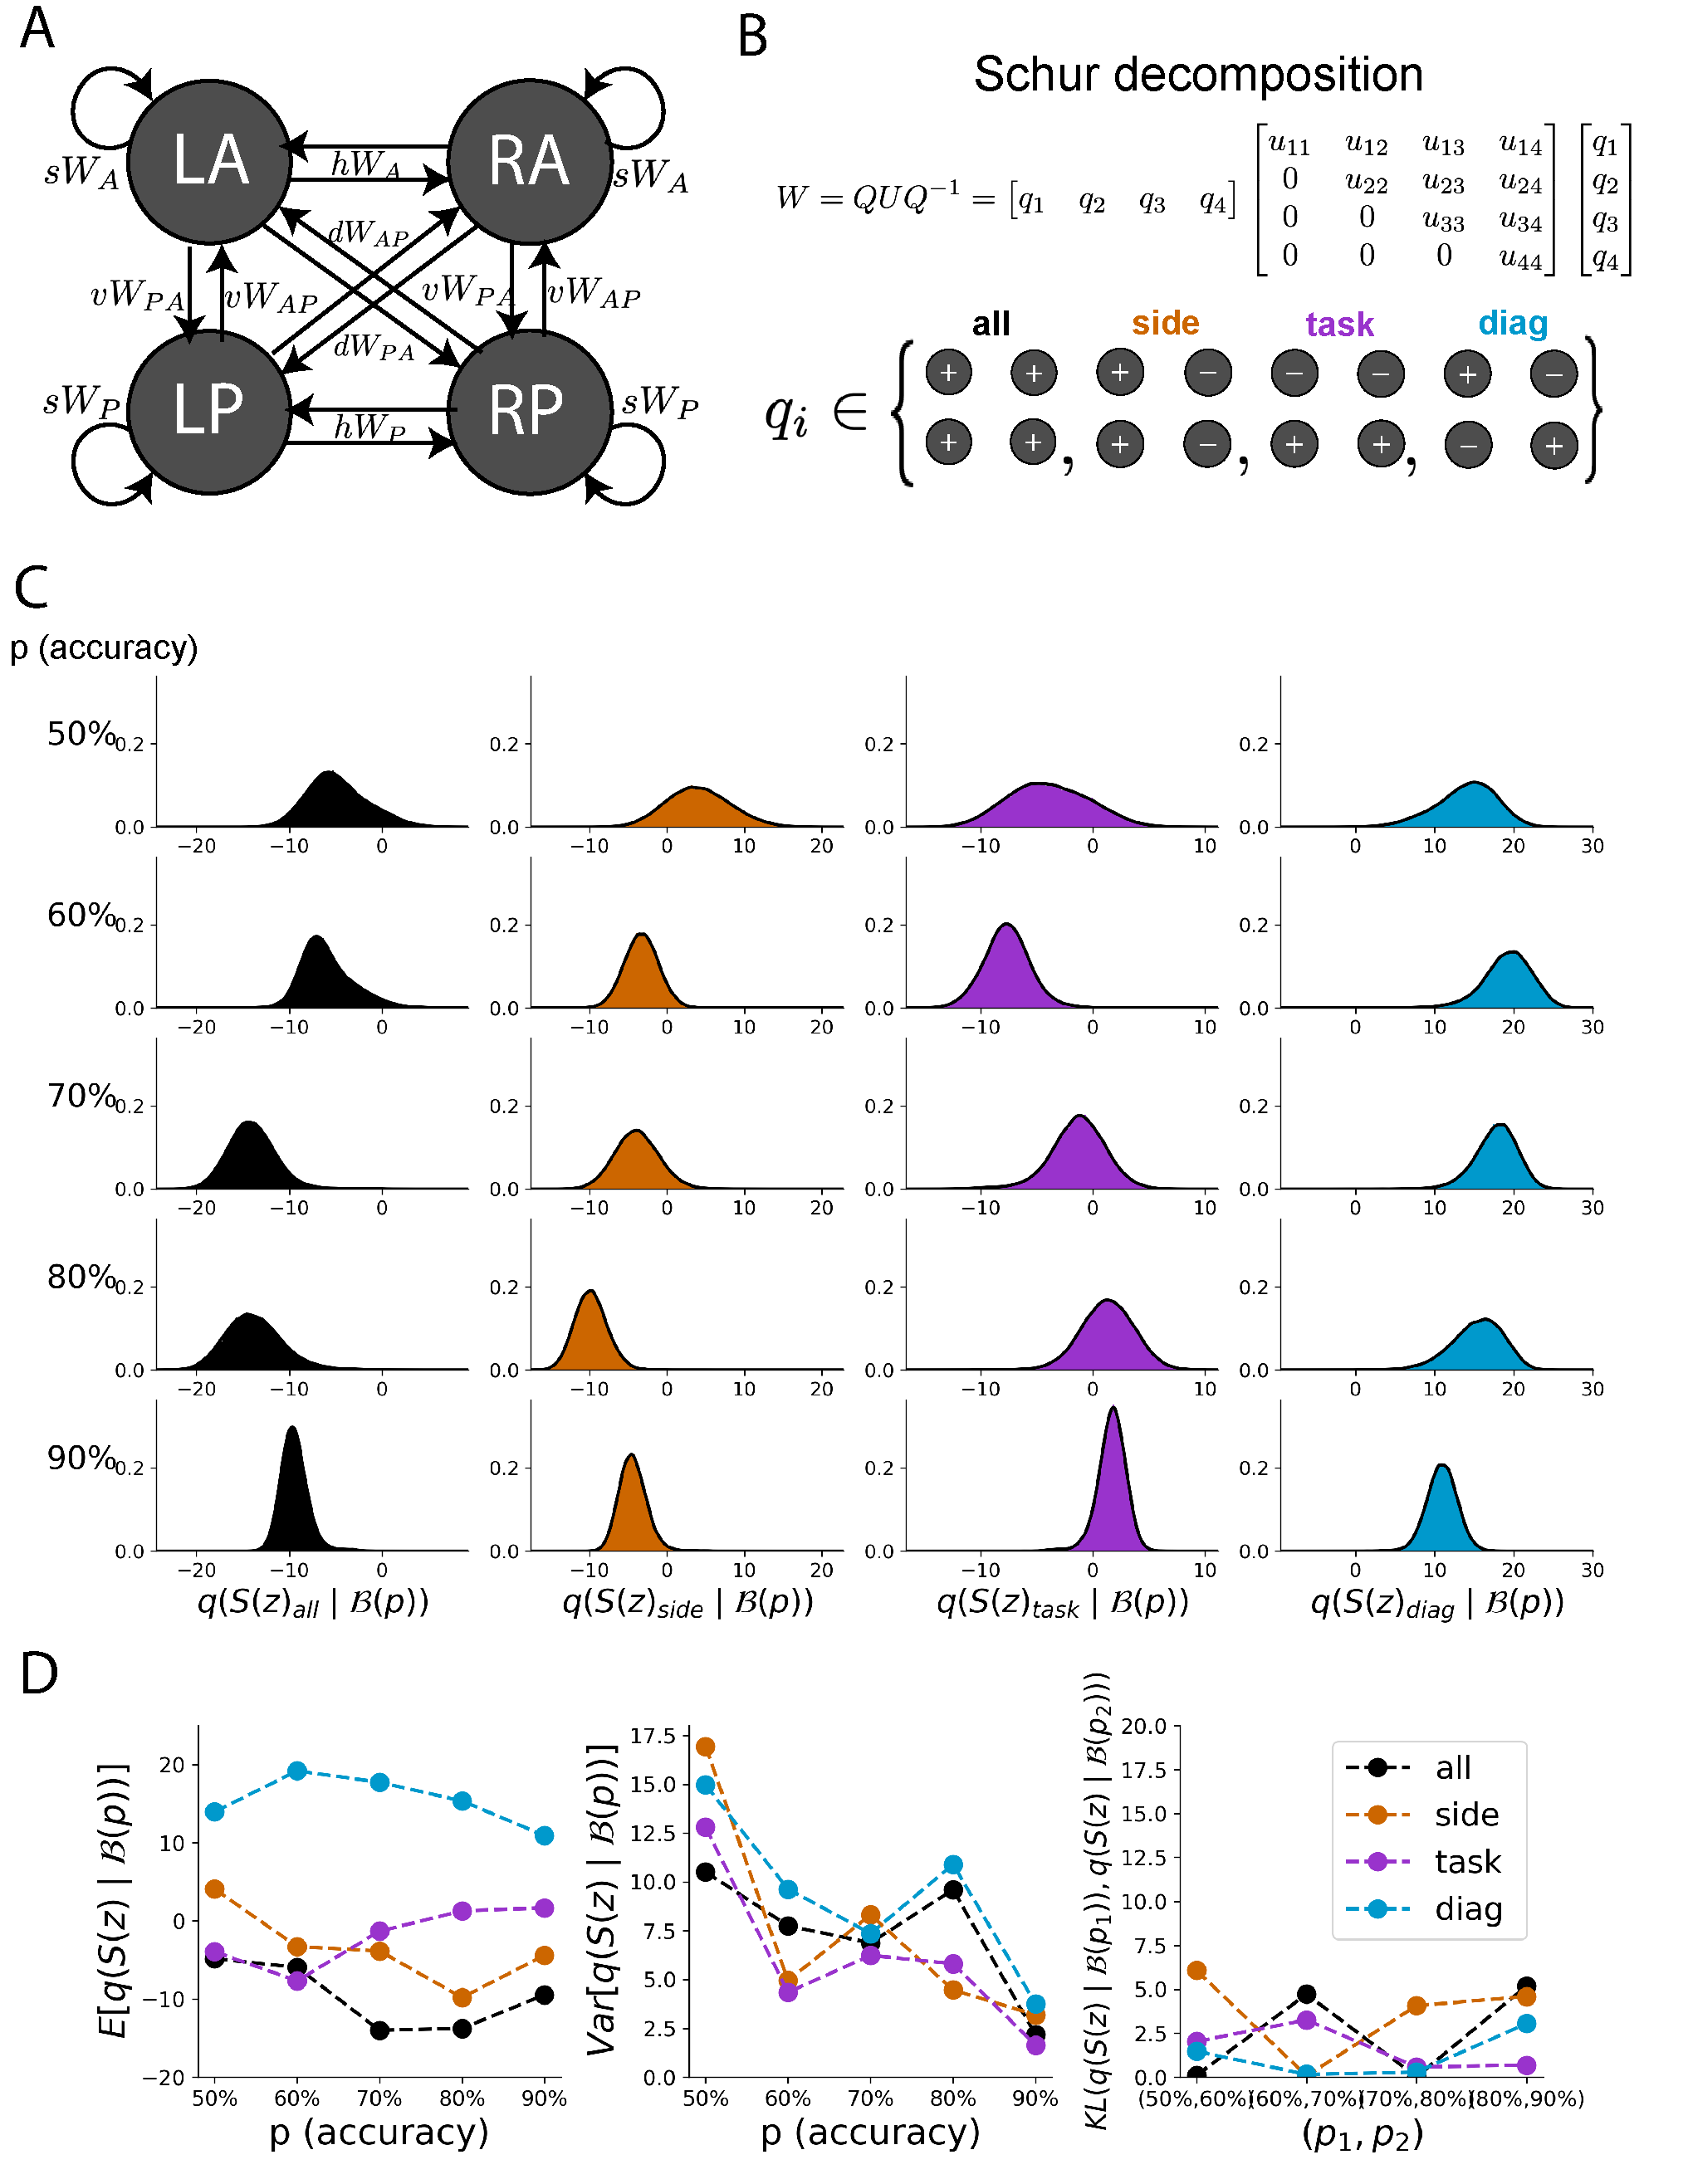
\includegraphics[scale=0.5]{models/SC/SC_Fig/SC_Fig.pdf}
\end{center}
\caption{\protectA.) Model of superior collicullus (SC). Neurons: LP - left pro, RP - right pro, LA - left anti, RA - right anti.  Parameters: sW - self, hW - horizontal, vW -vertical, dW - diagonal weights.  B.) Schur decomposition of W.  C.) DSN distribution of schur mode eigenvalues $S(z)$ with task learning.  D.) DSN means and variances (left and center, respectively) and step-wise KLs.}
\end{figure}
\end{document}

